\documentclass[12pt]{report}

% import and apply GIRS "formatting.sty" file
\usepackage{import}
\usepackage{formatting}

% source-code listings (used in Appendix A)
\usepackage{listings}
\lstset{
    basicstyle=\ttfamily\footnotesize,
    breaklines=true,
    showstringspaces=false,
    numbers=left,
    numberstyle=\tiny,
    frame=single,
    captionpos=b,
    language=Python,
    inputencoding=utf8,
    extendedchars=true,
    literate=
        {—}{{\textemdash}}1
        {–}{{\textendash}}1
        {…}{{\ldots}}1
        {'}{{\textquoteright}}1
        {'}{{\textquoteleft}}1
        {"}{{\textquotedblleft}}1
        {"}{{\textquotedblright}}1
}

% figures live in ./figures/
\graphicspath{{figures/}}

% [H] float placement -- keeps each screenshot pinned exactly where it
% is placed in the source instead of drifting to a later page (the
% default [h!] gives up and floats forward when a figure is nearly a
% full page tall, which is the case for most screenshots here).
\usepackage{float}

% load hyperref last to minimize conflicts
\usepackage{xcolor}
\usepackage[linktocpage=true]{hyperref}
\hypersetup{colorlinks=true, linkcolor=blue, citecolor=blue}

%-------------------------------------------------------
\begin{document}

%-------------------------------------------------------
\frontmatter
%-------------------------------------------------------
% TITLE PAGE
% Assignment requirement: "Start with identifying yourself
% and provide a title for your report."
%-------------------------------------------------------

\begin{center}
\vspace*{60pt}

{\fontsize{18pt}{0pt} \textbf{%
    Assignment 1
    % TODO: title of the report
    }}
\vspace*{100pt}

{\fontsize{14pt}{0pt} \textbf{%
    Fernando Melo Filho
    % TODO: your full name
    }}
\vspace*{2pt}

% {\fontsize{14pt}{0pt} \sf{%
%     <Student ID>
%     % TODO: student ID number
%     }}
% \vspace*{2pt}

{\fontsize{14pt}{0pt} \sf{%
    fmelofilho2950@floridapoly.edu
    % TODO: institutional email
    }}
\vspace*{24pt}

{\fontsize{14pt}{0pt} \textbf{%
    CAP 5410 --- Computer Vision
    }}

\vspace*{2pt}
{\fontsize{14pt}{0pt} \sf{%
    Assignment 1
    }}

\vspace*{24pt}
{\fontsize{14pt}{0pt} \sf{%
    Instructor: Dr. Muhammad Abid
    % TODO: instructor name
    }}

\vspace*{60pt}
{\fontsize{12pt}{0pt} \sf{%
    Brightness and Contrast Editing
    % TODO: e.g. subject of the lab
    }}

\vspace{\stretch{8}}

{\fontsize{12pt}{0pt} \sf{
    Department of Computer Science \\
    Florida Polytechnic University, Florida, USA }} \\
\vspace*{\fill}

{\fontsize{12pt}{0pt} \sf{
    September 2026
    % TODO: submission month and year
    }}

\end{center}
\thispagestyle{empty}

% \phantomsection
% % set up
\begin{center}
    {\fontsize{18pt}{0pt} \MakeUppercase{\textbf{abstract}}}
\vspace*{24pt}
\end{center}
\addcontentsline{toc}{chapter}{Abstract}
%-------------------------------------------------------

% TODO: one paragraph, one page maximum. Cover, in order:
%   - what the program does (dual video display + live histograms)
%   - the tools used (Python, OpenCV, Tkinter, NumPy, Pillow)
%   - the adjustments implemented (brightness, contrast)
%   - what was produced (saved edited video, persisted settings)
%   - the outcome / what was demonstrated

<ABSTRACT TEXT>

% \phantomsection
% % set up
\begin{center}
    {\fontsize{18pt}{0pt} \MakeUppercase{\textbf{acknowledgments}}}
\vspace*{24pt}
\end{center}
\addcontentsline{toc}{chapter}{Acknowledgments}
%-------------------------------------------------------

% TODO: brief. Credit course material, instructor, documentation
% consulted (OpenCV docs, Tkinter docs) and any peer discussion.
% Anything reused from an external source must also be cited in
% Chapter 2 and listed in references.bib.

<ACKNOWLEDGMENTS TEXT>


\phantomsection
\insertTOC
\setcounter{tocdepth}{2}

\phantomsection
\insertLOF

\phantomsection
\insertLOT

%-------------------------------------------------------
\mainmatter
\chapter{Introduction}
\label{ch:intro}

%-------------------------------------------------------

% TODO: 1-2 paragraphs framing the assignment: what problem is being
% solved and why video brightness/contrast adjustment with histogram
% feedback is a standard image-processing task.

%%%%%%%%%%%%%%%%%%%%%%%%%%%%%%%%%%%%%%%%%%%%%%%%%%%%%
\section{Objectives}
\label{sec:objectives}
%%%%%%%%%%%%%%%%%%%%%%%%%%%%%%%%%%%%%%%%%%%%%%%%%%%%%

The assignment requires implementing a program that satisfies the
following eight tasks:

\begin{enumerate}
  \item Load and display the source video.
  \item Display the histogram of the source video.
  \item Display the same video as an adjustable preview.
  \item Display the histogram of the preview video.
  \item Loop both videos continuously, so that each restarts from its
        first frame as soon as it ends.
  \item Provide brightness and contrast scroll bars.
  \item Provide a save function, triggered by a button, a key, or a
        key combination.
  \item Persist the adjusted settings so that, when the program is
        reloaded, both windows reopen with the previous settings
        already applied.
\end{enumerate}


%%%%%%%%%%%%%%%%%%%%%%%%%%%%%%%%%%%%%%%%%%%%%%%%%%%%%
\section{Background}
\label{sec:background}
%%%%%%%%%%%%%%%%%%%%%%%%%%%%%%%%%%%%%%%%%%%%%%%%%%%%%

Image processing can be described as a function that takes one or
more images as input and produces an image as output. Once an image
is loaded, its pixel values can be manipulated in a variety of ways.
These manipulations fall into two broad categories: point operators
and neighborhood operators \citep{szeliski2022}. In a point operator,
the value of an output pixel depends only on the value of the
corresponding input pixel; in a neighborhood operator, the output
pixel also depends on the pixels surrounding it.

Two of the most common point operations are multiplication and
addition by a constant, combined into a single expression:
\begin{equation}
  g(x) = \alpha \cdot f(x) + \beta
  \label{eq:pointop-1d}
\end{equation}
where $f$ is the input image and $g$ is the output image. Applied to
every pixel of a two-dimensional image (see Equation
\ref{eq:pointop}), the same operation is written as
\begin{equation}
  g(x,y) = \alpha \cdot f(x,y) + \beta
  \label{eq:pointop}
\end{equation}

The parameter $\alpha$ is called the \emph{gain} and controls
contrast, while $\beta$ is called the \emph{bias} and controls
brightness. A dark image has many low-intensity pixels, so its
histogram shows a peak toward the left (low) end. Adding a constant
bias shifts every pixel by the same amount, which translates the
whole histogram to the right for $\beta > 0$ or to the left for
$\beta < 0$. Because pixel intensities are stored as 8-bit values,
any result above 255 is clipped to 255 and any result below 0 is
clipped to 0.


%%%%%%%%%%%%%%%%%%%%%%%%%%%%%%%%%%%%%%%%%%%%%%%%%%%%%
\section{Report Organization}
\label{sec:organization}
%%%%%%%%%%%%%%%%%%%%%%%%%%%%%%%%%%%%%%%%%%%%%%%%%%%%%

The remainder of this report is organized as follows. Chapter
\ref{ch:method} describes the development environment, the
application architecture, and how each of the eight tasks was
implemented. Chapter \ref{ch:results} presents sample outputs of the
program for each task. Chapter \ref{ch:conclusion} discusses the
results, notes the limitations encountered, and concludes the report.
   % Introduction
\chapter{Methodology and Implementation}
\label{ch:method}

%-------------------------------------------------------

% TODO: opening paragraph. State the language, libraries and why they
% were chosen (OpenCV for decoding/histograms, Tkinter for the GUI and
% scroll bars, NumPy for array work, Pillow to bridge OpenCV -> Tkinter).
% Note that MATLAB was not used, as required.




%%%%%%%%%%%%%%%%%%%%%%%%%%%%%%%%%%%%%%%%%%%%%%%%%%%%%
\section{Development Environment}
\label{sec:environment}
%%%%%%%%%%%%%%%%%%%%%%%%%%%%%%%%%%%%%%%%%%%%%%%%%%%%%

Table \ref{table:environment} lists the language and libraries I used
to build and run the program, with their versions. Video capture,
writing, and histogram computation all go through OpenCV
\citep{bradski2000}; array operations use NumPy
\citep{harris2020numpy}; frames are converted for display with
Pillow \citep{pillow}; and the interface is built with Tkinter
\citep{tkinter}.

\begin{table}[h]
    \centering
    \caption[Software environment.]%
    {Software environment used to develop and run the program.}

    \begin{tabular}{P{1.6in}|P{1.2in}|P{2.4in}}
        \specialrule{1.5pt}{0pt}{0pt}
        Component & Version & Purpose \\
        \hline\hline
        Python & 3.13.5 & Programming language used to implement the application \\
        \specialrule{0.5pt}{0pt}{0pt}
        OpenCV (opencv-python) & 5.0.0.93 & Video capture and writing, frame processing, and histogram computation \\
        \specialrule{0.5pt}{0pt}{0pt}
        NumPy & 2.5.2 & Array operations \\
        \specialrule{0.5pt}{0pt}{0pt}
        Pillow (PIL) & 12.3.0 & Converts OpenCV BGR frames into images that Tkinter can display \\
        \specialrule{0.5pt}{0pt}{0pt}
        Tkinter & bundled with Python (Tcl/Tk) & GUI toolkit: windows, scroll bars, buttons and labels \\
        \specialrule{1.5pt}{0pt}{0pt}
    \end{tabular}
    \label{table:environment}
\end{table}


%%%%%%%%%%%%%%%%%%%%%%%%%%%%%%%%%%%%%%%%%%%%%%%%%%%%%
\section{Application Architecture}
\label{sec:architecture}
%%%%%%%%%%%%%%%%%%%%%%%%%%%%%%%%%%%%%%%%%%%%%%%%%%%%%

% TODO: describe the overall structure -- the single class, the UI build
% step, the frame loop, and the separation between the display pipeline
% and the export pipeline.


I implemented the whole application as a single class,
\texttt{VideoEditor} (Listing \ref{lst:architecture-class}), and
grouped its methods by responsibility, as shown in Table
\ref{table:methods}.

\lstinputlisting[language=Python, firstline=41, lastline=44,
    firstnumber=auto,
    caption={The \texttt{VideoEditor} class and constructor signature (\texttt{main.py}).},
    label={lst:architecture-class}]{../main.py}

\begin{table}[h]
    \centering
    \caption[Key methods of the \texttt{VideoEditor} class.]%
    {Key methods of the \texttt{VideoEditor} class and their responsibility.}

    \begin{tabular}{P{1.6in}|P{3.6in}}
        \specialrule{1.5pt}{0pt}{0pt}
        Method & Responsibility \\
        \hline\hline
        \texttt{\_\_init\_\_} & Opens the source video, restores persisted settings, builds the UI, and starts the main loop \\
        \specialrule{0.5pt}{0pt}{0pt}
        \texttt{\_build\_ui} / \texttt{\_video\_column} & Construct the video panels, histogram panels, sliders, and buttons \\
        \specialrule{0.5pt}{0pt}{0pt}
        \texttt{\_process} & Applies the brightness/contrast point operation (Equation \ref{eq:pointop}) to a frame \\
        \specialrule{0.5pt}{0pt}{0pt}
        \texttt{\_hist\_image} & Renders a per-channel histogram into a small BGR canvas \\
        \specialrule{0.5pt}{0pt}{0pt}
        \texttt{\_show} & Converts a BGR frame into a Tkinter-displayable image \\
        \specialrule{0.5pt}{0pt}{0pt}
        \texttt{\_read\_looping} / \texttt{\_tick} & Timer-driven main loop: reads frames, loops at end of stream, and refreshes all four panels \\
        \specialrule{0.5pt}{0pt}{0pt}
        \texttt{\_load\_settings} / \texttt{\_store\_settings} & Read and write \texttt{settings.json} to persist slider values between runs \\
        \specialrule{0.5pt}{0pt}{0pt}
        \texttt{\_save} / \texttt{\_save\_worker} / \texttt{\_poll\_save} & Prompt for an output file, export it on a background thread, and report progress \\
        \specialrule{0.5pt}{0pt}{0pt}
        \texttt{\_toggle\_pause} / \texttt{\_reset} / \texttt{close} & Pause/resume playback, reset the sliders, and release resources on exit \\
        \specialrule{1.5pt}{0pt}{0pt}
    \end{tabular}
    \label{table:methods}
\end{table}

% Optional: a block diagram / window-layout figure matching the layout
% required by the assignment brief.
\begin{figure}[H]
    \centering
    % \includegraphics[width = 0.8\textwidth]{<architecture_diagram>}
    \caption[Application architecture.]%
    {<Caption: block diagram of the processing pipeline and window layout.>}
    \label{fig:architecture}
\end{figure}


%%%%%%%%%%%%%%%%%%%%%%%%%%%%%%%%%%%%%%%%%%%%%%%%%%%%%
\section{Task 1 --- Loading and Displaying the Source Video}
\label{sec:task1}
%%%%%%%%%%%%%%%%%%%%%%%%%%%%%%%%%%%%%%%%%%%%%%%%%%%%%

% TODO: how the file is opened, how frames are read, how a BGR frame
% becomes a widget image, and how the failure case is handled.


I open the source file once, in the constructor, with
\texttt{cv2.VideoCapture}; if the file cannot be opened, I show an
error dialog and close the window (Listing \ref{lst:task1-open}).

\lstinputlisting[language=Python, firstline=46, lastline=55,
    firstnumber=auto,
    caption={Opening the source video and computing the display size (\texttt{main.py}).},
    label={lst:task1-open}]{../main.py}

Every decoded frame is a NumPy array in OpenCV's BGR channel order,
so to display it inside a Tkinter label I convert it to RGB and wrap
it in a \texttt{PIL.ImageTk.PhotoImage}~\citep{pillow} (Listing
\ref{lst:task1-show}). I keep a reference to the image in
\texttt{self.\_refs}, since Tkinter does not hold its own reference
and would otherwise garbage-collect it and leave the panel blank.

\lstinputlisting[language=Python, firstline=263, lastline=267,
    firstnumber=auto,
    caption={Converting a BGR frame into a Tkinter-displayable image (\texttt{main.py}).},
    label={lst:task1-show}]{../main.py}


%%%%%%%%%%%%%%%%%%%%%%%%%%%%%%%%%%%%%%%%%%%%%%%%%%%%%
\section{Task 2 --- Histogram of the Source Video}
\label{sec:task2}
%%%%%%%%%%%%%%%%%%%%%%%%%%%%%%%%%%%%%%%%%%%%%%%%%%%%%

% TODO: how the per-channel histogram is computed, how many bins, how it
% is normalized to the canvas height, and how it is drawn and refreshed
% once per frame.


For each of the three color channels, I use
\texttt{cv2.calcHist}~\citep{bradski2000} to bin the frame into 256 bins
over the range $[0,256)$, normalize the result to the height of the
histogram canvas, and draw it as a polyline (Listing
\ref{lst:task2-hist}).

\lstinputlisting[language=Python, firstline=248, lastline=261,
    firstnumber=auto,
    caption={Computing and drawing the per-channel histogram (\texttt{main.py}).},
    label={lst:task2-hist}]{../main.py}

I call this routine once per tick for the original frame, so the
histogram panel refreshes at the same rate as the video (Listing
\ref{lst:task2-call}).

\lstinputlisting[language=Python, firstline=303, lastline=304,
    firstnumber=auto,
    caption={Refreshing the original video's histogram panel every frame (\texttt{main.py}).},
    label={lst:task2-call}]{../main.py}


%%%%%%%%%%%%%%%%%%%%%%%%%%%%%%%%%%%%%%%%%%%%%%%%%%%%%
\section{Task 3 --- Preview (Adjusted) Video}
\label{sec:task3}
%%%%%%%%%%%%%%%%%%%%%%%%%%%%%%%%%%%%%%%%%%%%%%%%%%%%%

% TODO: explain that a single decoded frame feeds both panels, that the
% right panel is the adjusted copy, and why the two stay in sync.


Both panels come from the same decoded frame, so they can never fall
out of sync: I get the right-hand (``Edited'') panel by applying a
brightness/contrast point operation to a copy of that frame with
\texttt{cv2.convertScaleAbs} (Listing \ref{lst:task3-process}), which
computes the linear mapping and clips the result to $[0,255]$ in one
call.

\lstinputlisting[language=Python, firstline=231, lastline=246,
    firstnumber=auto,
    caption={The brightness/contrast point operation, centered on mid-gray, applied to a frame (\texttt{main.py}).},
    label={lst:task3-process}]{../main.py}

\lstinputlisting[language=Python, firstline=298, lastline=299,
    firstnumber=auto,
    caption={Building the adjusted (preview) frame once per tick (\texttt{main.py}).},
    label={lst:task3-call}]{../main.py}


%%%%%%%%%%%%%%%%%%%%%%%%%%%%%%%%%%%%%%%%%%%%%%%%%%%%%
\section{Task 4 --- Histogram of the Preview Video}
\label{sec:task4}
%%%%%%%%%%%%%%%%%%%%%%%%%%%%%%%%%%%%%%%%%%%%%%%%%%%%%

% TODO: same routine applied to the adjusted frame; explain what the
% viewer should expect to see happen to the distribution as each slider
% moves (shift vs. stretch, and clipping at the ends of the range).

I reuse the same \texttt{\_hist\_image} routine from Section
\ref{sec:task2} on the adjusted frame, so both histograms are always
computed identically and only differ because of the
brightness/contrast operation itself (Listing \ref{lst:task4-call}).

\lstinputlisting[language=Python, firstline=305, lastline=306,
    firstnumber=auto,
    caption={Refreshing the preview video's histogram panel every frame (\texttt{main.py}).},
    label={lst:task4-call}]{../main.py}


%%%%%%%%%%%%%%%%%%%%%%%%%%%%%%%%%%%%%%%%%%%%%%%%%%%%%
\section{Task 5 --- Continuous Looping Playback}
\label{sec:task5}
%%%%%%%%%%%%%%%%%%%%%%%%%%%%%%%%%%%%%%%%%%%%%%%%%%%%%

% TODO: how end-of-stream is detected, how the position is rewound to
% frame 0, and how the timed callback drives playback at the target rate.

\texttt{cv2.VideoCapture.read} returns \texttt{False} once the last
frame has been consumed; when that happens, \texttt{\_read\_looping}
rewinds the capture to frame 0 with \texttt{CAP\_PROP\_POS\_FRAMES}
and reads again, so playback never stops (Listing
\ref{lst:task5-read}).

\lstinputlisting[language=Python, firstline=271, lastline=278,
    firstnumber=auto,
    caption={Reading the next frame and rewinding to frame 0 at end of stream (\texttt{main.py}).},
    label={lst:task5-read}]{../main.py}

I drive playback with \texttt{\_tick}, a callback that Tkinter's
event loop re-invokes every \texttt{FRAME\_DELAY} ($30$~ms, $\approx
33$~fps) through \texttt{root.after}. Each call reads one frame from
each capture, builds the four panels described in Sections
\ref{sec:task1}--\ref{sec:task4}, and reschedules itself, which is
what keeps both videos playing continuously (Listing
\ref{lst:task5-tick}).

\lstinputlisting[language=Python, firstline=280, lastline=308,
    firstnumber=auto,
    caption={The timer-driven main loop that keeps both videos playing continuously (\texttt{main.py}).},
    label={lst:task5-tick}]{../main.py}


%%%%%%%%%%%%%%%%%%%%%%%%%%%%%%%%%%%%%%%%%%%%%%%%%%%%%
\section{Task 6 --- Brightness and Contrast Scroll Bars}
\label{sec:task6}
%%%%%%%%%%%%%%%%%%%%%%%%%%%%%%%%%%%%%%%%%%%%%%%%%%%%%

% TODO: the two sliders, their ranges and defaults, the variable each is
% bound to, and how a slider change reaches the next rendered frame.
% Reference Equation \ref{eq:pointop} from Chapter 1.

I built the two scroll bars as \texttt{ttk.Scale}~\citep{tkinter}
widgets bound to the \texttt{tk.DoubleVar} instances
\texttt{self.brightness} and
\texttt{self.contrast} (Listing \ref{lst:task6-sliders}). Because
\texttt{\_process} (Listing \ref{lst:task3-process}) reads these
variables directly every tick, moving a slider takes effect on the
very next rendered frame, with no extra event wiring needed.

\lstinputlisting[language=Python, firstline=170, lastline=182,
    firstnumber=auto,
    caption={Brightness and contrast scroll bars (\texttt{main.py}).},
    label={lst:task6-sliders}]{../main.py}

Table \ref{table:controls} lists the range and default of each
control, corresponding to $\alpha$ and $\beta$ in Equation
\ref{eq:pointop}.

\begin{table}[h]
    \centering
    \caption[Adjustment controls.]%
    {Adjustment controls, their ranges and their effect on the image.}

    \begin{tabular}{P{1.2in}|c|c|P{2.6in}}
        \specialrule{1.5pt}{0pt}{0pt}
        Control & Symbol & Range (default) & Effect \\
        \hline\hline
        Brightness & $\beta$ & $-100$ to $100$ ($0$) & Additive offset: shifts every pixel intensity up or down, translating the histogram left or right; clipped to $[0,255]$ \\
        \specialrule{0.5pt}{0pt}{0pt}
        Contrast & $\alpha$ & $0.1$ to $3.0$ ($1.0$) & Multiplicative gain pivoted on mid-gray (127.5): $\alpha>1$ stretches the histogram outward from the center (higher contrast), $\alpha<1$ compresses it toward the center (lower contrast), without shifting the overall brightness; also clipped to $[0,255]$ \\
        \specialrule{1.5pt}{0pt}{0pt}
    \end{tabular}
    \label{table:controls}
\end{table}


%%%%%%%%%%%%%%%%%%%%%%%%%%%%%%%%%%%%%%%%%%%%%%%%%%%%%
\section{Task 7 --- Save Functionality}
\label{sec:task7}
%%%%%%%%%%%%%%%%%%%%%%%%%%%%%%%%%%%%%%%%%%%%%%%%%%%%%

% TODO: how saving is triggered, the codec/container written, why the
% source is re-read at full resolution instead of exporting the preview,
% why the export runs off the UI thread, and how progress and errors are
% reported.

I trigger saving either from the ``Save Video\ldots'' button or with
\texttt{Ctrl+S} (both bound in the constructor, Listing
\ref{lst:architecture-class}). I snapshot the current $\alpha$ and
$\beta$ values at that moment, so later slider movements do not
affect an export already in progress (Listing \ref{lst:task7-save}).

\lstinputlisting[language=Python, firstline=321, lastline=341,
    firstnumber=auto,
    caption={Triggering the save dialog and starting the export on a background thread (\texttt{main.py}).},
    label={lst:task7-save}]{../main.py}

The export re-opens the source file at full resolution, instead of
reusing the down-scaled preview frames, and runs on a background
thread so both video panels keep updating while it works (Listings
\ref{lst:task7-setup} and \ref{lst:task7-loop}).

\lstinputlisting[language=Python, firstline=343, lastline=357,
    firstnumber=auto,
    caption={Re-opening the source at full resolution and preparing the output writer (\texttt{main.py}, excerpt).},
    label={lst:task7-setup}]{../main.py}

\lstinputlisting[language=Python, firstline=359, lastline=366,
    firstnumber=auto,
    caption={Applying the settings to each frame and tracking export progress (\texttt{main.py}, excerpt).},
    label={lst:task7-loop}]{../main.py}

\texttt{\_poll\_save} (Listing \ref{lst:task7-poll}) is the only
place I touch Tkinter widgets while the export runs; the worker
thread only ever writes to plain instance attributes
(\texttt{self.save\_progress}, \texttt{self.save\_error}), which
keeps me from touching Tkinter from the wrong thread.

\lstinputlisting[language=Python, firstline=376, lastline=394,
    firstnumber=auto,
    caption={Polling the export status from the UI thread and reporting the result (\texttt{main.py}).},
    label={lst:task7-poll}]{../main.py}


%%%%%%%%%%%%%%%%%%%%%%%%%%%%%%%%%%%%%%%%%%%%%%%%%%%%%
\section{Task 8 --- Persisting Settings Across Restarts}
\label{sec:task8}
%%%%%%%%%%%%%%%%%%%%%%%%%%%%%%%%%%%%%%%%%%%%%%%%%%%%%

% TODO: where the slider values are stored between runs, the file format,
% when they are written, when they are read back, and the fallback when
% no stored settings exist.

I store brightness, contrast, and the path of the last exported file
in a JSON file, \texttt{settings.json}, next to the script.
\texttt{\_load\_settings} reads it back when the program starts, and
\texttt{\_store\_settings} writes it whenever the program closes and
again right after a successful save, so both windows reopen with the
same brightness, contrast, and exported-video source as before.

\lstinputlisting[language=Python, firstline=88, lastline=109,
    firstnumber=auto,
    caption={Reading and writing \texttt{settings.json} (\texttt{main.py}).},
    label={lst:task8-persist}]{../main.py}

\lstinputlisting[language=Python, firstline=396, lastline=400,
    firstnumber=auto,
    caption={Settings are written back when the window closes (\texttt{main.py}).},
    label={lst:task8-close}]{../main.py}


%%%%%%%%%%%%%%%%%%%%%%%%%%%%%%%%%%%%%%%%%%%%%%%%%%%%%
\section{Additional Features}
\label{sec:extras}
%%%%%%%%%%%%%%%%%%%%%%%%%%%%%%%%%%%%%%%%%%%%%%%%%%%%%

Table \ref{table:extras} lists a few features I added beyond the
eight required tasks.

\begin{table}[h]
    \centering

    \begin{tabular}{P{1.7in}|P{1.3in}|P{2.0in}}
        \specialrule{1.5pt}{0pt}{0pt}
        Feature & Implemented in & Trigger \\
        \hline\hline
        Pause / resume playback & \texttt{\_toggle\_pause} & ``Pause'' button or spacebar \\
        \specialrule{0.5pt}{0pt}{0pt}
        Reset sliders to defaults & \texttt{\_reset} & ``Reset'' button \\
        \specialrule{0.5pt}{0pt}{0pt}
        Save keyboard shortcut & \texttt{\_save} & \texttt{Ctrl+S} \\
        \specialrule{0.5pt}{0pt}{0pt}
        Export progress bar & \texttt{\_poll\_save} & Updates automatically while saving \\
        \specialrule{0.5pt}{0pt}{0pt}
        Toggle left panel between the original source and the last exported video & \texttt{\_toggle\_saved} & ``Left panel: exported video'' checkbox \\
        \specialrule{1.5pt}{0pt}{0pt}
    \end{tabular}
    \caption[Additional features.]%
    {Features implemented beyond the eight required tasks.}
    \label{table:extras}
\end{table}


%%%%%%%%%%%%%%%%%%%%%%%%%%%%%%%%%%%%%%%%%%%%%%%%%%%%%
\section{Requirements Traceability}
\label{sec:traceability}
%%%%%%%%%%%%%%%%%%%%%%%%%%%%%%%%%%%%%%%%%%%%%%%%%%%%%

Table \ref{table:traceability} maps each of the eight required tasks
to the function(s) that implement it and to the figure in Chapter
\ref{ch:results} that demonstrates it.

\begin{table}[h]
    \centering
    \caption[Requirements traceability.]%
    {Mapping of each assignment requirement to its implementation and to the figure that demonstrates it.}

    \begin{tabular}{c|P{1.9in}|P{1.7in}|c}
        \specialrule{1.5pt}{0pt}{0pt}
        \# & Requirement & Implemented in & Evidence \\
        \hline\hline
        1 & Load video on screen & \texttt{\_\_init\_\_}, \texttt{\_show} & Fig.~\ref{fig:default} \\
        \specialrule{0.5pt}{0pt}{0pt}
        2 & Histogram of that video & \texttt{\_hist\_image} & Fig.~\ref{fig:default} \\
        \specialrule{0.5pt}{0pt}{0pt}
        3 & Same video as preview & \texttt{\_process} & Fig.~\ref{fig:default} \\
        \specialrule{0.5pt}{0pt}{0pt}
        4 & Histogram of the preview & \texttt{\_hist\_image} & Fig.~\ref{fig:default} \\
        \specialrule{0.5pt}{0pt}{0pt}
        5 & Continuous looping & \texttt{\_read\_looping}, \texttt{\_tick} & Fig.~\ref{fig:looping} \\
        \specialrule{0.5pt}{0pt}{0pt}
        6 & Brightness / contrast bars & \texttt{\_build\_ui} & Figs.~\ref{fig:brightness}, \ref{fig:contrast} \\
        \specialrule{0.5pt}{0pt}{0pt}
        7 & Save functionality & \texttt{\_save}, \texttt{\_save\_worker} & Fig.~\ref{fig:save} \\
        \specialrule{0.5pt}{0pt}{0pt}
        8 & Settings restored on reload & \texttt{\_load\_settings}, \texttt{\_store\_settings} & Fig.~\ref{fig:persistence} \\
        \specialrule{1.5pt}{0pt}{0pt}
    \end{tabular}
    \label{table:traceability}
\end{table}
   % Methodology / Implementation  (Tasks 1-8)
\chapter{Results}
\label{ch:results}

%-------------------------------------------------------

% TODO: opening paragraph. Name the input video, its resolution, frame
% rate and length, and state which settings each screenshot below uses.
% Assignment requirement: "Include samples of outputs of your program."

%%%%%%%%%%%%%%%%%%%%%%%%%%%%%%%%%%%%%%%%%%%%%%%%%%%%%
\section{Input Video}
\label{sec:input}
%%%%%%%%%%%%%%%%%%%%%%%%%%%%%%%%%%%%%%%%%%%%%%%%%%%%%

\begin{table}[h]
    \centering
    \caption[Input video properties.]%
    {Properties of the input video used for all results in this chapter.}

    \begin{tabular}{P{2.2in}|P{2.2in}}
        \specialrule{1.5pt}{0pt}{0pt}
        Property & Value \\
        \hline\hline
        File name & \texttt{barriers.avi} \\
        \specialrule{0.5pt}{0pt}{0pt}
        Resolution (W $\times$ H) & $640 \times 480$ \\
        \specialrule{0.5pt}{0pt}{0pt}
        Frame rate & 50 fps \\
        \specialrule{0.5pt}{0pt}{0pt}
        Frame count & 399 \\
        \specialrule{0.5pt}{0pt}{0pt}
        Duration & $\approx 8.0$ s \\
        \specialrule{0.5pt}{0pt}{0pt}
        Codec / container & FMP4 / AVI \\
        \specialrule{1.5pt}{0pt}{0pt}
    \end{tabular}
    \label{table:inputvideo}
\end{table}


%%%%%%%%%%%%%%%%%%%%%%%%%%%%%%%%%%%%%%%%%%%%%%%%%%%%%
\section{Main Window at Default Settings}
\label{sec:res-default}
%%%%%%%%%%%%%%%%%%%%%%%%%%%%%%%%%%%%%%%%%%%%%%%%%%%%%

% Covers Tasks 1-4: both videos and both histograms visible at once.
% TODO: describe what the screenshot shows and why the two histograms
% are identical at default settings.

\begin{figure}[H]
    \centering
    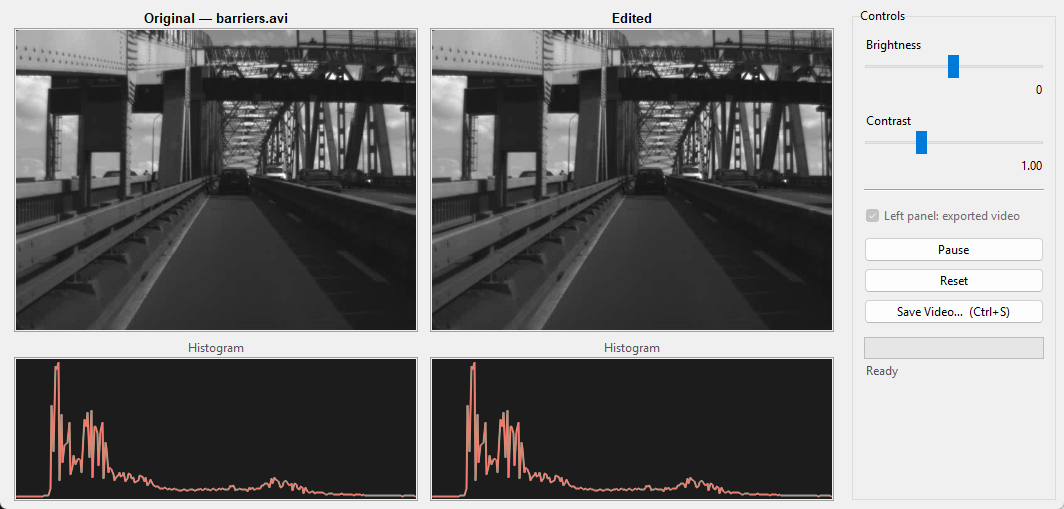
\includegraphics[width = \textwidth]{screenshot_default.png}
    \caption[Main window at default settings.]%
    {Full application window at the default settings ($\beta=0$,
    $\alpha=1.0$): the original video (left) and the preview video
    (right) with their respective histograms underneath, plus the
    control panel.}
    \label{fig:default}
\end{figure}


%%%%%%%%%%%%%%%%%%%%%%%%%%%%%%%%%%%%%%%%%%%%%%%%%%%%%
\section{Effect of the Brightness Control}
\label{sec:res-brightness}
%%%%%%%%%%%%%%%%%%%%%%%%%%%%%%%%%%%%%%%%%%%%%%%%%%%%%

% Covers Task 6 (brightness half).
% TODO: state the slider value used in each subfigure and describe the
% shift of the histogram, including any clipping.

\begin{figure}[H]
    \centering
    \begin{subfigure}{0.48\linewidth}
        \centering
        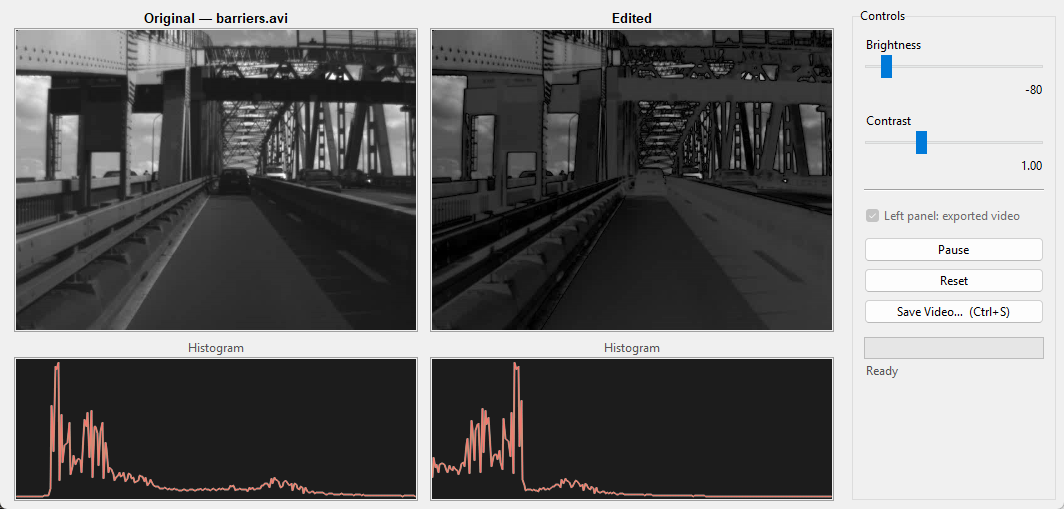
\includegraphics[width=\textwidth]{screenshot_brightness_low.png}
        \caption{$\beta = -80$}
        \label{fig:bright-low}
    \end{subfigure}
    \hfill
    \begin{subfigure}{0.48\linewidth}
        \centering
        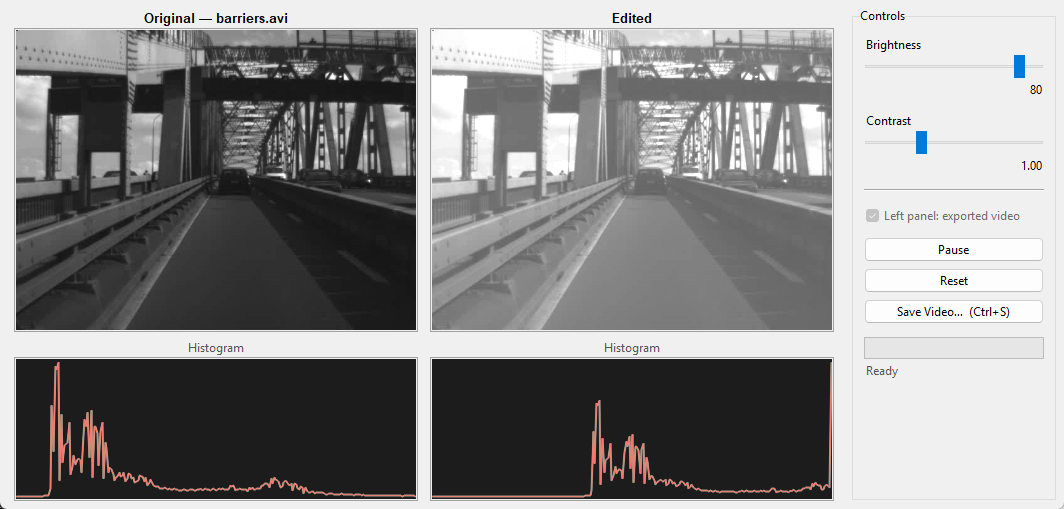
\includegraphics[width=\textwidth]{screenshot_brightness_high.png}
        \caption{$\beta = +80$}
        \label{fig:bright-high}
    \end{subfigure}
    \caption[Effect of the brightness control.]%
    {Preview video and its histogram at two brightness settings
    ($\alpha=1.0$ fixed in both), compared against the unmodified
    original on the left of each panel. The histogram translates left
    for negative $\beta$ and right for positive $\beta$, exactly as
    described in Table \ref{table:controls}.}
    \label{fig:brightness}
\end{figure}


%%%%%%%%%%%%%%%%%%%%%%%%%%%%%%%%%%%%%%%%%%%%%%%%%%%%%
\section{Effect of the Contrast Control}
\label{sec:res-contrast}
%%%%%%%%%%%%%%%%%%%%%%%%%%%%%%%%%%%%%%%%%%%%%%%%%%%%%

% Covers Task 6 (contrast half).
% TODO: state the slider value used in each subfigure and describe the
% stretching or compression of the histogram.

\begin{figure}[H]
    \centering
    \begin{subfigure}{0.48\linewidth}
        \centering
        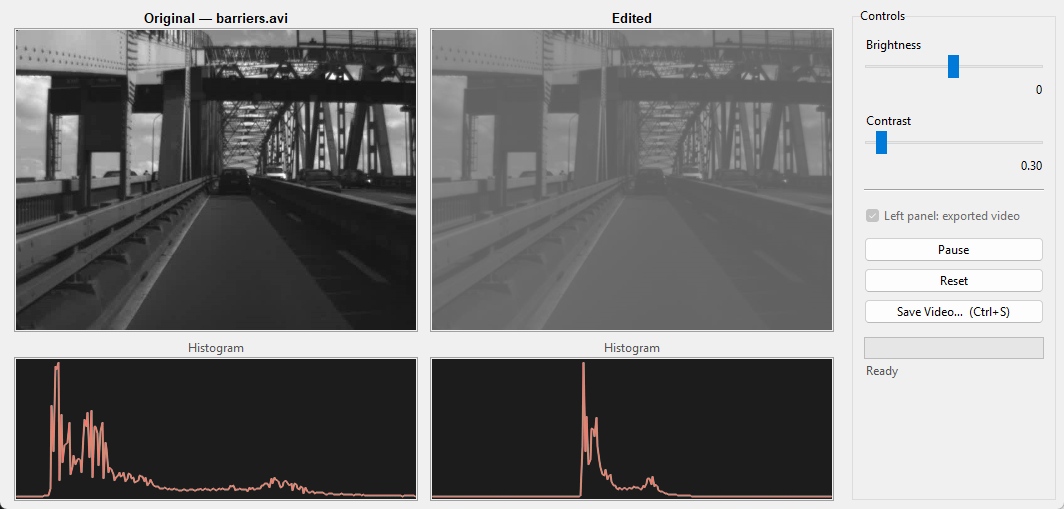
\includegraphics[width=\textwidth]{screenshot_contrast_low.png}
        \caption{$\alpha = 0.3$}
        \label{fig:contrast-low}
    \end{subfigure}
    \hfill
    \begin{subfigure}{0.48\linewidth}
        \centering
        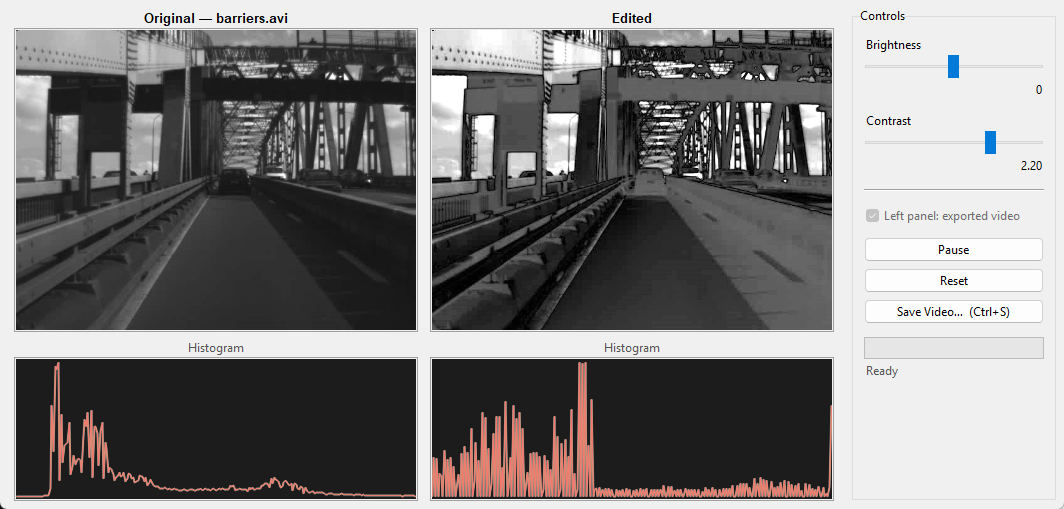
\includegraphics[width=\textwidth]{screenshot_contrast_high.png}
        \caption{$\alpha = 2.2$}
        \label{fig:contrast-high}
    \end{subfigure}
    \caption[Effect of the contrast control.]%
    {Preview video and its histogram at two contrast settings
    ($\beta=0$ fixed in both), compared against the unmodified
    original on the left of each panel. At $\alpha=0.3$ the histogram
    compresses toward mid-gray; at $\alpha=2.2$ it spreads out and
    several bins clip at 0 and 255.}
    \label{fig:contrast}
\end{figure}


%%%%%%%%%%%%%%%%%%%%%%%%%%%%%%%%%%%%%%%%%%%%%%%%%%%%%
\section{Continuous Playback}
\label{sec:res-loop}
%%%%%%%%%%%%%%%%%%%%%%%%%%%%%%%%%%%%%%%%%%%%%%%%%%%%%

% Covers Task 5.
% TODO: show the last frame and the restarted first frame, or describe
% how looping was verified.

\begin{figure}[H]
    \centering
    \begin{subfigure}{0.48\linewidth}
        \centering
        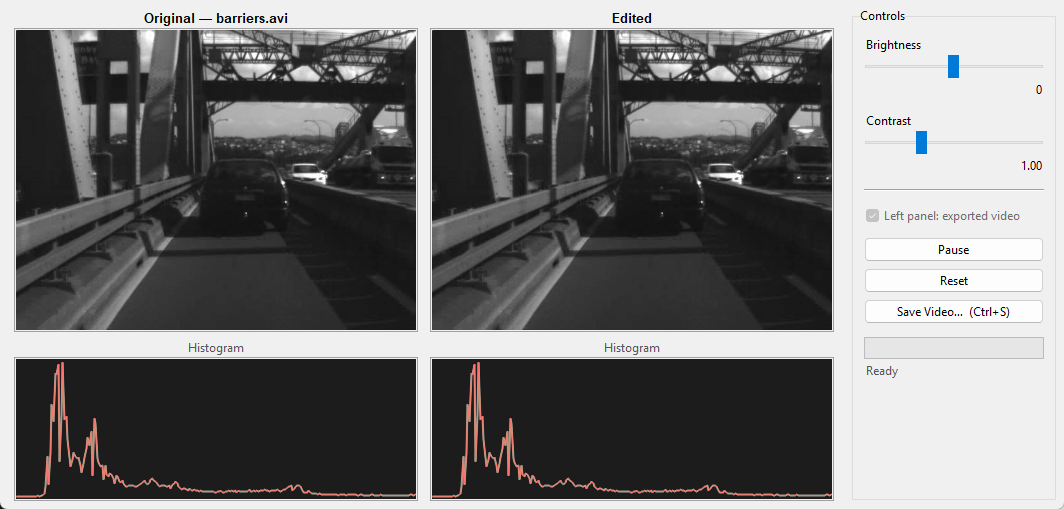
\includegraphics[width=\textwidth]{screenshot_loop_last.png}
        \caption{Frame 399 (final frame)}
        \label{fig:loop-last}
    \end{subfigure}
    \hfill
    \begin{subfigure}{0.48\linewidth}
        \centering
        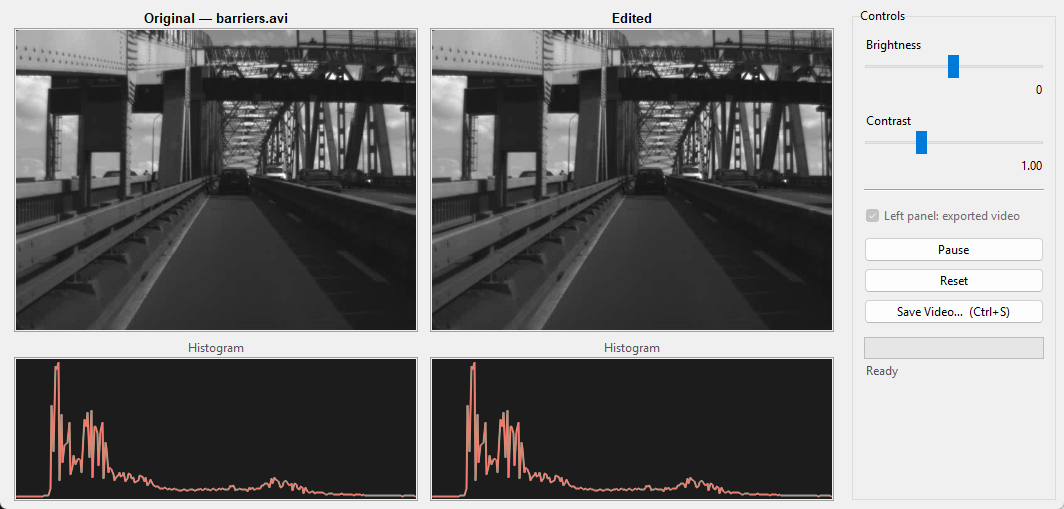
\includegraphics[width=\textwidth]{screenshot_loop_first.png}
        \caption{Frame 1, immediately after the automatic restart}
        \label{fig:loop-first}
    \end{subfigure}
    \caption[Automatic restart at end of stream.]%
    {Playback wrapping from the final frame of \texttt{barriers.avi}
    back to frame 1 without any user action, exercising the same
    end-of-stream/rewind path (\texttt{\_read\_looping}, Listing
    \ref{lst:task5-read}) shown in Section \ref{sec:task5}.}
    \label{fig:looping}
\end{figure}


%%%%%%%%%%%%%%%%%%%%%%%%%%%%%%%%%%%%%%%%%%%%%%%%%%%%%
\section{Saving the Adjusted Video}
\label{sec:res-save}
%%%%%%%%%%%%%%%%%%%%%%%%%%%%%%%%%%%%%%%%%%%%%%%%%%%%%

% Covers Task 7.
% TODO: show the save dialog / progress / confirmation, and report the
% output file name, size and export time.

\begin{figure}[H]
    \centering
    \begin{subfigure}{0.48\linewidth}
        \centering
        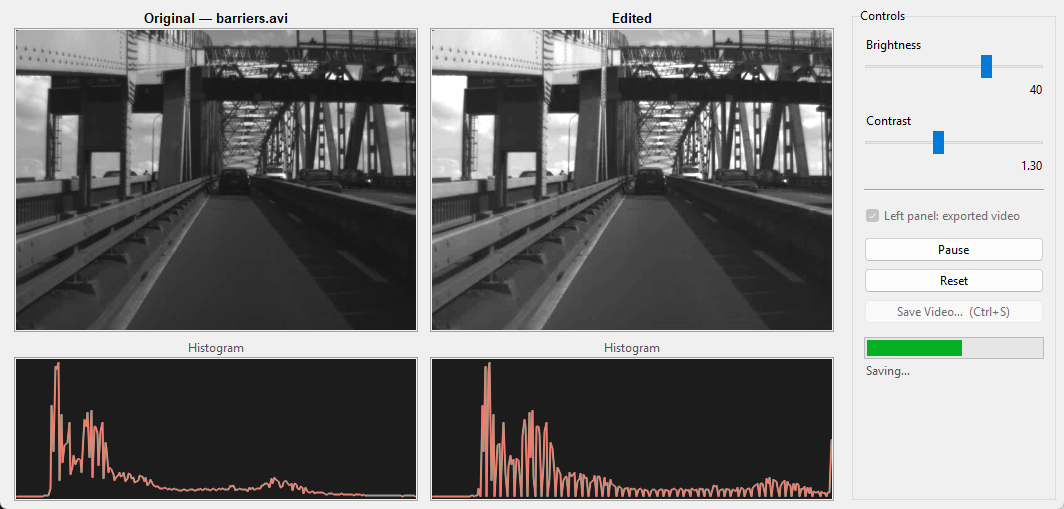
\includegraphics[width=\textwidth]{screenshot_save_progress.png}
        \caption{Export in progress}
        \label{fig:save-progress}
    \end{subfigure}
    \hfill
    \begin{subfigure}{0.48\linewidth}
        \centering
        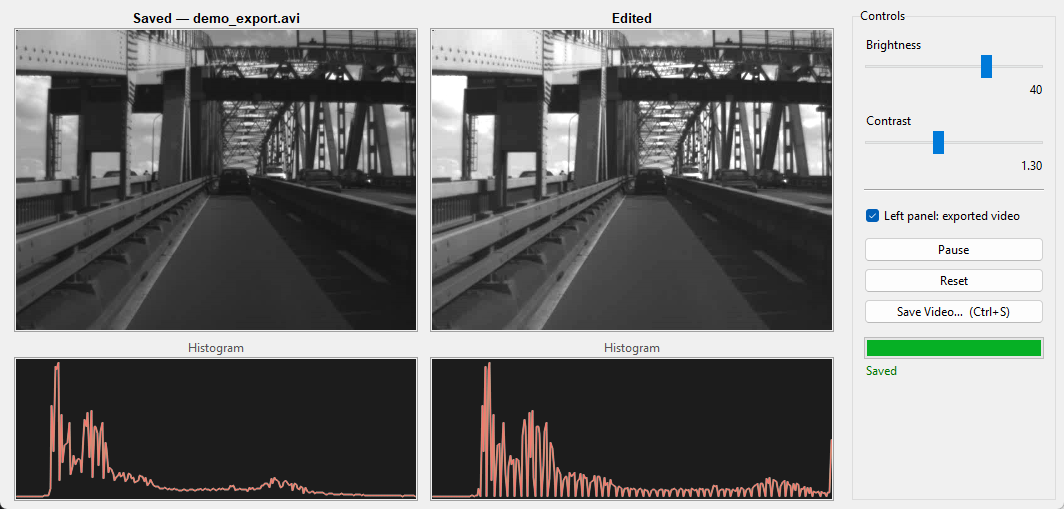
\includegraphics[width=\textwidth]{screenshot_save_done.png}
        \caption{Export complete}
        \label{fig:save-done}
    \end{subfigure}
    \caption[Save operation.]%
    {Saving with $\beta=40$, $\alpha=1.3$: (a) the ``Save Video\ldots''
    button disabled and the progress bar advancing while
    \texttt{\_save\_worker} re-encodes the source on a background
    thread; (b) after completion, the status reads ``Saved'' and the
    left panel automatically switches to play back the exported file
    (caption updates to ``Saved --- demo\_export.avi'').}
    \label{fig:save}
\end{figure}


%%%%%%%%%%%%%%%%%%%%%%%%%%%%%%%%%%%%%%%%%%%%%%%%%%%%%
\section{Settings Restored After Reload}
\label{sec:res-persist}
%%%%%%%%%%%%%%%%%%%%%%%%%%%%%%%%%%%%%%%%%%%%%%%%%%%%%

% Covers Task 8.
% TODO: before/after a restart -- same slider positions, same appearance
% in both windows.

\begin{figure}[H]
    \centering
    \begin{subfigure}{0.48\linewidth}
        \centering
        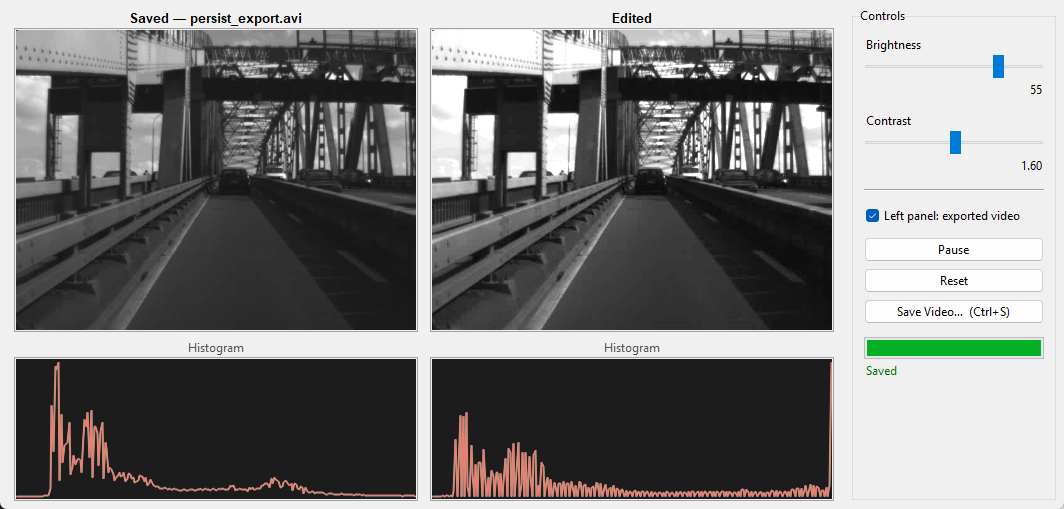
\includegraphics[width=\textwidth]{screenshot_persist_before.png}
        \caption{Before closing the program}
        \label{fig:persist-before}
    \end{subfigure}
    \hfill
    \begin{subfigure}{0.48\linewidth}
        \centering
        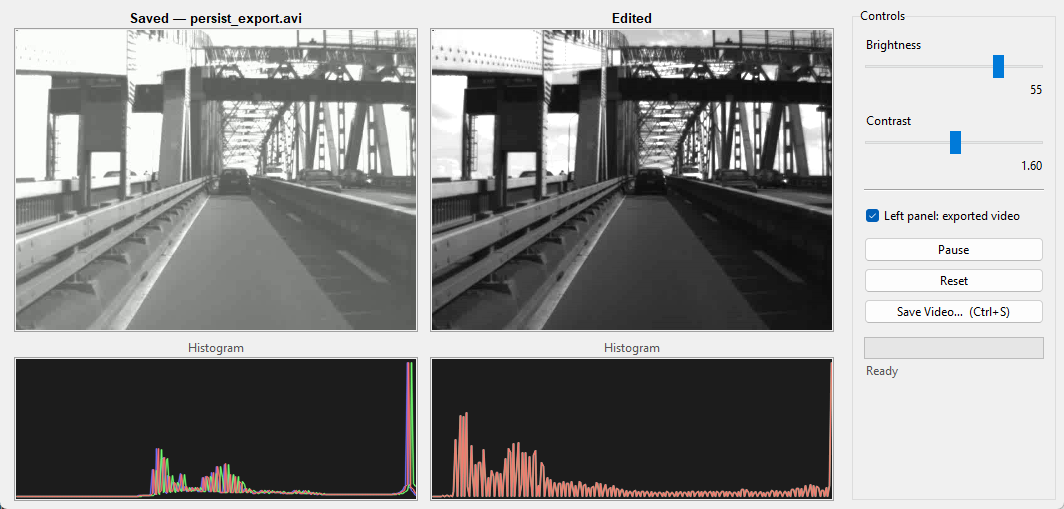
\includegraphics[width=\textwidth]{screenshot_persist_after.png}
        \caption{After restarting the program}
        \label{fig:persist-after}
    \end{subfigure}
    \caption[Settings restored on reload.]%
    {Brightness ($\beta=55$), contrast ($\alpha=1.6$), and the
    exported-video checkbox are all identical before closing (a) and
    immediately after a fresh launch (b), confirming that
    \texttt{settings.json} (Listing \ref{lst:task8-persist}) round-trips
    correctly.}
    \label{fig:persistence}
\end{figure}
   % Results  (program output samples)
\chapter{Discussion and Conclusion}
\label{ch:conclusion}

%-------------------------------------------------------

%%%%%%%%%%%%%%%%%%%%%%%%%%%%%%%%%%%%%%%%%%%%%%%%%%%%%
\section{Discussion}
\label{sec:discussion}
%%%%%%%%%%%%%%%%%%%%%%%%%%%%%%%%%%%%%%%%%%%%%%%%%%%%%

% TODO: interpret the results. Suggested points:
%   - what the histogram comparison reveals about the point operation
%   - where information is lost (saturation / clipping) and why
%   - performance: does the display keep up with the source frame rate

As a software engineer, I like to split every project into a backend part and a frontend part; separating them from the start lets me reason about the two sets of technologies independently. By the backend I mean the calculations that change the image's settings --- vector multiplication and so on. To actually see the result, rather than just debugging from the console, a frontend is needed. After some research, Tkinter was chosen because it is very simple to use: for now the interface only needs to be functional, and Tkinter gets the job done while keeping the code simple.


%%%%%%%%%%%%%%%%%%%%%%%%%%%%%%%%%%%%%%%%%%%%%%%%%%%%%
\section{Challenges and Limitations}
\label{sec:limitations}
%%%%%%%%%%%%%%%%%%%%%%%%%%%%%%%%%%%%%%%%%%%%%%%%%%%%%

% TODO: be honest and specific. Problems encountered, how each was
% resolved, and what the program still does not handle.
The main challenge was finding and organizing the functions needed to perform the operations. It ended up being a matter of identifying the right OpenCV (\texttt{cv2}) function for each task: \texttt{cv2.VideoCapture} and \texttt{cv2.VideoWriter} to read and write the video files, \texttt{cv2.calcHist} to build the histograms, \texttt{cv2.convertScaleAbs} to apply the brightness/contrast point operation with built-in clipping to $[0,255]$, and \texttt{cv2.resize}/\texttt{cv2.cvtColor} to prepare each frame for display. After that, the next challenge was connecting these results to the UI. OpenCV frames are NumPy arrays in BGR channel order, while Tkinter widgets can only display \texttt{PhotoImage} objects, so each frame had to be converted to RGB and wrapped with \texttt{PIL.ImageTk.PhotoImage} before it could be shown on a \texttt{Label} --- and a reference to that image had to be kept alive manually (Section \ref{sec:task1}), since Tkinter does not hold its own reference and would otherwise garbage-collect the image and leave the panel blank.


%%%%%%%%%%%%%%%%%%%%%%%%%%%%%%%%%%%%%%%%%%%%%%%%%%%%%
\section{Conclusion}
\label{sec:conclusion}
%%%%%%%%%%%%%%%%%%%%%%%%%%%%%%%%%%%%%%%%%%%%%%%%%%%%%

Brightness and contrast are point operations: they depend only on the input pixel to calculate the output. In this assignment, we showed how this works by adding sliders that change the video's brightness and contrast in real time, and observed how the histogram changes according to the values assigned to gain and bias.
   % Discussion and Conclusion

%-------------------------------------------------------
\backmatter
\bibliographystyle{ascelike}
\bibliography{references}

\begin{appendices}
\appendix
\addtocontents{toc}{\protect\setcounter{tocdepth}{0}}
\addtocontents{toc}{\protect\renewcommand{%
    \protect\chapterprefix}{%
    \protect\hspace*{-0.5in}APPENDIX\protect\hspace*{0.6in}}}%

%%%%%%%%%%%%%%%%%%%%%%%%%%%%%%%%%%%%%%%%%%%%%%%%%%%%%
%%% APPENDIX CONTENTS
%%%%%%%%%%%%%%%%%%%%%%%%%%%%%%%%%%%%%%%%%%%%%%%%%%%%%

\chapter{Source Code}
\label{app:source}

The complete, unmodified contents of \texttt{main.py} are listed
below; this is the same file submitted alongside this report. The
source code, the input video, and a README are also available at
\url{https://github.com/Fernando12filho/Brightness-Contrast-Display}.

\section{main.py}
\label{app:mainpy}

% Pulled in directly so the listing can never drift from the code
% that was actually submitted.
\lstinputlisting[language=Python, caption={Complete source code (\texttt{main.py}).}, label={lst:main}]{../main.py}
   % Full source code
% %%%%%%%%%%%%%%%%%%%%%%%%%%%%%%%%%%%%%%%%%%%%%%%%%%%%%
%%% APPENDIX TITLE PAGE
%%%%%%%%%%%%%%%%%%%%%%%%%%%%%%%%%%%%%%%%%%%%%%%%%%%%%

\begin{center}
\vspace*{60pt}

{\fontsize{18pt}{0pt} \MakeUppercase{\textbf{%
    Appendix B
    }}}
\vspace*{24pt}

{\fontsize{18pt}{0pt} \MakeUppercase{\textbf{%
    Installation and Usage
    }}}

\vspace*{100pt}
\end{center}
\thispagestyle{empty}

%%%%%%%%%%%%%%%%%%%%%%%%%%%%%%%%%%%%%%%%%%%%%%%%%%%%%
%%% APPENDIX CONTENTS
%%%%%%%%%%%%%%%%%%%%%%%%%%%%%%%%%%%%%%%%%%%%%%%%%%%%%

\chapter{Installation and Usage}
\label{app:usage}

\section{Contents of the Submitted Archive}
\label{app:archive}

% TODO: list every file in the zip (source, video, requirements, report
% PDF) with a one-line description of each.

\begin{itemize}
  \item <file> --- <description>
  \item <file> --- <description>
  \item <file> --- <description>
\end{itemize}

\section{Dependencies}
\label{app:deps}

% TODO: the install command and the pinned versions.

<DEPENDENCIES TEXT>

\section{Running the Program}
\label{app:run}

% TODO: the exact command to run, and what the user should expect on
% screen once it starts.

<RUN INSTRUCTIONS TEXT>

\section{Controls}
\label{app:controls}

% TODO: table or list of every control and keyboard shortcut.

\begin{itemize}
  \item <control> --- <what it does>
  \item <control> --- <what it does>
  \item <control> --- <what it does>
\end{itemize}
   % How to run / environment
\end{appendices}


\end{document}
%-------------------------------------------------------
